\documentclass[12pt,letterpaper]{article}

\usepackage{amsmath, amsthm, amssymb, amsfonts}
\usepackage{graphicx}
\usepackage{bm}
\usepackage{natbib}

\theoremstyle{definition}
\newtheorem{dfn}{Definition}

\begin{document}

% The numbers below controls the amount of space between the following sections
\def\shiftdowna{0.32in}  % Adjust for balance
\def\shiftdownb{0.22in}  % Adjust for balance



\begin{center}
\textbf{{\large Project Work Statement}}\\


% SPONSOR
\vspace \shiftdowna
\underline {Sponsor}\\ 
\vspace{5pt}
\textbf{{\large JABRE CAPITAL PARTNERS}}\\


% TITLE
\vspace \shiftdowna
\textbf{{\large Improving return performance and divisifying stock selections}}


% STUDENTS
\vspace{0.35in}
\vspace \shiftdownb
\underline {Participants} \\
\vspace{5pt}
\text{Tianyu Luo}, \texttt{tluo3@jhu.edu}

% SPONSORS
\vspace \shiftdownb
\underline {Potential Participants}\\
\vspace{5pt}
\text{Zichan Wang}, \texttt{zichang.wang@gmail.com} \\
\vspace{3pt}
\text{Yue Meng}, \texttt{mengyue902@gmail.com} \\
\vspace{3pt}
%\text{Glen Coppersmith}, \texttt{coppersmith@jhu.edu}

% DATE
\vspace \shiftdowna
Date: \today

\end{center}

\vfill  
%Fill page to force following note to bottom
\footnoterule
\noindent \small{Any apparent association of this work to Jabre Capital Partners is
fictional one, and the sole purpose of this work is a class exercise}

\newpage

\section{Background} 
Jabre Capital Partners is an alternative asset management platform founded in 2006. The Group offers a diversified range of investment management services and products, including Cayman-based collective investment schemes, UCITS IV regulated strategies, and individually managed accounts, to a broad network of institutional and high net worth clients. In addition, the Group provides discretionary investment management and advisory services to private clients.

As of December 31th 2010, Jabre Capital had portfolio value of \$4,133,365,000. A year later, the portfolio value was only \$793,966,000.In one year, the hedge fund's value was down by around 80\%, which made it among the 10 worst hedge funds 2011.   

\section{Problem Statement}
Figure 1 implies that Philippe Jabre, the fund manager, changed stocks of the portfolio from quater to quarter. Sadly, his judgements did not prevent the portfolio value from skyfalling. According  to the talk with Mr. Jabre, he changed stocks frequently was because he wanted to be conservative and reduce risk through diversification. Besides, due to the low portfolio value, Mr. Jabre was limited to invest in large numbers of stocks to increase diversification.

%Thus, our task will be as follows:
%\begin{itemize}
%\item We should tell Mr. Jabre whether his portfolio is truly diversified or not,
%\item We should help Mr. Jabre narrow down his stock selection.
%\end{itemize}
\begin{figure}[h]
    \begin{center}
        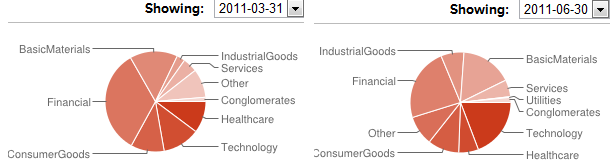
\includegraphics[width=\textwidth]{../images/1.png}
    \end{center}
 %   \caption{Jabre Capital's Portfolio Selection in 2011}
    \label{fig:piechart}
\end{figure}  
\begin{figure}[h]
    \begin{center}
        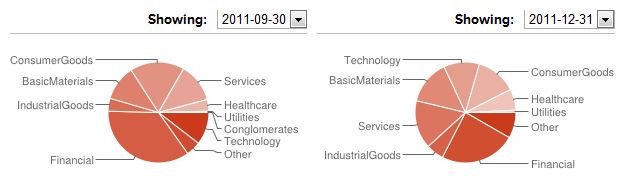
\includegraphics[width=\textwidth]{../images/2.png}
    \end{center}
    \caption{Jabre Capital's Portfolio Selection in 2011}
    \label{fig:piechart}
\end{figure}  
\newpage
According to our conversation, Mr. Jabre had difficulties in technical analysis( finding support and resistance lines, and then decide to call and put). Besides, Mr. Jabre did not get the recipe for diversification. Actually, a large number of different stocks doesn't gurantee diversification. Diversification is aimed at decreasing risk of a portfolio by introducing diversified stocks. If stocks are positively related to each other, the portfolio risk increases rather than decreases.

We can also see Mr. Jabre changed industry percentage in his portfolio. From Sep 30 to Dec 31 2011, Mr. Jabre decreased the percentage of stocks in finance, and increased the percentage of stocks in industrial goods. Mr.Jabre understood that it was not necessary to invest in a large number of stocks in the same industry. For example, the bank stocks are positively correlated when the monetary policies are not favorable. Then the question comes to which industries we can reduce the number of stocks Jabre Capital hold, and which industries we can focus our investment in one stock because a specific stock has already explained a certain pattern of stock performance in this industry? Stock performance is influenced by macro econmic environment factors shared by all the companies, and individual company factors which is case sentitive. Macro econimic environment factors are the ones which cause the universal pattern in a given industry. Unfortunately, these factors are mixed with individual company factors. It is complex for us to decide whether we can just invest in one stock to represent the whole industry.

 \section{Approach}
In our approach of task 1, firstly we should know the concept of support and resistance lines. 
\begin{itemize}
\item Support is the price level at which demand is thought to be strong enough to prevent the price from declining further, 
\item Resistance is the price level at which selling is thought to be strong enough to prevent the price from rising further.
\end{itemize}
If we can find lines where the price won't go above or below, they are support and resistance lines.

Thus, my approach is as follows:
\begin{itemize}
\item Find points where the  derivative is about to change signal,
\item Find the maximum and minimum point among the points above,
\item Among all the points where the derivative is going to be positive, draw a line which conects minimum point and another point with the smallest absolute value of slope rate,
\item Among all the points where the derivative is going to be negative, draw a line which conects maximum point and another point with the smallest absolute value of slope rate.
\end{itemize}

In our approach of task 2 and 3, we will use the return performance of a stock rather than price peformance, as the thing we are interested in is changes in the stock price rather than absolute stock prices.
Thus, to help Jabre Capital with its challenges, our approach will be divided into following steps:
\begin{itemize}
\item Develop a software which can automatically draw support and resistance lines in a given period of time,
\item Get historical prices of stocks ever on Jabre Capital's list in 2011, and develop historical return ratios accordingly,
\item Divide stocks accroding to industries they are in, and list important macro econimic factors(such as matrial prices) to a specific industry,
\item Gather historical data of the macro econimic factors, and decide whether these factors are favorable to stock performance or not,
\item If macro econimc fators are favorable or neutral to a certain industry, apply Principal Component Analysis to find whether there is a specific return pattern in the industry,
	\begin{itemize}
	\item If there is a certain pattern, elect one stock with highest average return ratio and minimized risk to represent a specific industry,
	\item If there is no such pattern, divide stocks in the same industry into subcatogries to find whether there is a certain pattern or not, until the number of stocks in this industry decreases by 80\% which corresponds to the portfolio value loss.
	\end{itemize}
\item If macro ecnomic factors are not favorable to a certain industry, decide whether to exit this industry or not, by referring to authorized third party opnions about the factor's future trends.
\end{itemize} 

\section{Milestones}
We have the following major deadlines:
\begin{itemize}
    \item Work Statement due date, Oct 1, 2012,
    \item Midterm Presentation due date, Oct 17, 2012,
    \item Progress Report due date, Oct 26, 2012,
    \item Final Presentation due date, Nov 6, 2012,
    \item Final Report due date, Nov 30, 2012.
\end{itemize}
\section{Deliverable}
\subsection{From Team to Sponsor} % (fold)
The following outputs are expected from this project:
\begin{itemize}
    \item Software of finding support and resistance line,
    \item Return of Investment charts and data of all the stocks Jabre Capital invested in 2011,
    \item Principal component analysis of all the stocks, stocks in each industry, stocks in each subcategory,
    \item Suggestions about a narrowed portfolio list,
    \item R package with a complete set of documentations along with some test codes that can be used to reproduce simulation results,
    \item Technical report and presentations summarizing the work. 
\end{itemize}

\subsection{From Sponsor to Team} % (fold)

In order for our project to be of successful one, we will need:
\begin{itemize}
    \item Provide lists of stocks Jabre Capital held in 2011, and access to all the price charts and data of these stocks before Oct 26,2012
     \item Timely responses to inquiries, 
    \item Symposium attendance travel expenses.
\end{itemize}


%\newpage
%\bibliographystyle{plain}
%%\renewcommand\bibname{Selected Bibliography Including Cited Works}
%\nocite{*}
%\bibliography{biblio}

\end{document}

